\addcontentsline{etoc}{chapter}{\textit{Kudryavtsev I.\,V., Gorgadze V.\,V., Belenov A.\,V.} Secure Storage and Recovery of User Data Using Multi-Agent Scheme in Cosmos}%

\begin{abstract}
Решение проблемы уязвимости пользователей к потере приватных ключей для безопасного хранения и восстановления данных в блокчейн-системах является критически важным, так как потеря ключа означает безвозвратную утрату доступа к данным и цифровым активам. Предложен метод восстановления зашифрованных данных через группу доверенных лиц, основанный на математическом алгоритме разделения секрета Шамира. Ключ делится на части и распределяется между участниками так, что для восстановления требуется согласие минимального числа из них. Система реализована для блокчейна Cosmos и обеспечивает защиту от компрометации отдельных участников при сохранении возможности восстановления данных. Решение не требует доверия к централизованным сервисам и подтверждено экспериментально на работающем прототипе.

\kwr блокчейн, Cosmos, схема Шамира, абстракция аккаунта, восстановление ключей, мультиагентная система

\blfootnote{\hspace{-7pt}\textcopyright \, Кудрявцев И.\,В., Горгадзе В.\,В., Беленов А.\,В., 2025\\ \indent\textcopyright \, Федеральное государственное автономное образовательное учреждение высшего образования\\
\indent\hspace{15pt}<<Московский физико-технический институт
(национальный исследовательский университет)>>, 2025}

\end{abstract}

\arthead{I.\,V. Kudryavtsev$^{1}$, V.\,V. Gorgadze$^{1}$, A.\,V. Belenov$^{1}$}
{$^{1}$Moscow Institute of Physics and Technology (National Research University)\par}
{Secure Storage and Recovery of User Data Using Multi-Agent Scheme in Cosmos}

\begin{abstract}
Solving the problem of user vulnerability to private key loss for secure storage and data recovery in blockchain systems is critically important, as key loss means irreversible loss of access to data and digital assets. A method for recovering encrypted data through a group of trusted parties is proposed, based on Shamir's Secret Sharing mathematical algorithm. The key is divided into shares and distributed among participants so that recovery requires agreement of a minimum number of them. The system is implemented for Cosmos blockchain and provides protection against compromise of individual participants while maintaining data recovery capability. The solution requires no trust in centralized services and is experimentally validated on a working prototype.

\kwe blockchain, Cosmos, Shamir's scheme, account abstraction, key recovery, multi-agent system
\end{abstract}
\bigskip


\section{Введение}

Развитие децентрализованных технологий и блокчейн-сетей открыло новые горизонты в области цифровой идентичности и управления пользовательскими данными. Однако вместе с этим появились и новые вызовы, связанные с безопасностью и сохранностью доступа к данным. Одной из ключевых проблем остаётся высокая уязвимость пользователей к потере приватных ключей, которая в традиционных блокчейн-системах означает полную и безвозвратную утрату доступа к аккаунту и связанным с ним цифровым активам и конфиденциальным данным.

Современные подходы к решению этой проблемы включают механизмы:
\begin{enumerate}
\item
социального восстановления (social recovery)~--- передачу части полномочий по восстановлению доверенной группе лиц;

\item
абстракции аккаунта (account abstraction)~--- реализацию аутентификации и авторизации через программируемую логику смарт-контрактов.
\end{enumerate}

Несмотря на перспективность этих решений, существующие реализации зачастую ограничиваются восстановлением лишь доступа к управлению аккаунтом, но не охватывают проблему восстановления зашифрованных пользовательских данных. Кроме того, они требуют предварительной конфигурации и не всегда обеспечивают должный уровень безопасности в сценариях с частичной компрометацией доверенных участников.

Цель данной работы~--- разработка и реализация расширенного подхода к безопасному хранению и восстановлению пользовательских данных в экосистеме \textbf{Cosmos}. Предлагаемое решение сочетает в себе мультиагентную схему на основе социальной модели доверия с использованием алгоритма разделения секрета Шамира (\textbf{Shamir Secret Sharing}) и хранением зашифрованного ключа непосредственно в состоянии смарт-контракта. Такая архитектура позволяет пользователю не только гибко управлять доступом, но и восстанавливать утраченные зашифрованные данные даже при потере собственного ключа, опираясь на сеть доверенных лиц.

\subsection{Научный и практический вклад}

Основной вклад работы:

\begin{enumerate}
\item
Формализована пороговая модель восстановления зашифрованных пользовательских данных (в отличие от существующих подходов, ограничивающихся восстановлением доступа к аккаунту и активам) на основе интеграции схемы Шамира и механизма социального восстановления в архитектуру абстрактного аккаунта экосистемы Cosmos. Модель обеспечивает полную децентрализацию через сеть независимых guardians без зависимости от Web2-провайдеров.

\item
Проведён количественный анализ безопасности и отказоустойчивости: доказана конфиденциальность при компрометации до $k-1$ участников и функциональность при отказе до $n-k$ участников для конфигурации $(k,n)$-пороговой схемы.

\item
Реализован и экспериментально подтверждён работоспособный прототип на базе \textbf{CosmWasm} с открытым исходным кодом на локальной тестовой сети \textbf{Cosmos SDK}, демонстрирующий практическую применимость предложенного подхода.
\end{enumerate}

Принципиальное отличие от аналогов: Argent Wallet~\cite{s1} восстанавливает доступ к аккаунту и активам, Leap/Keplr используют централизованные OAuth-провайдеры, но ни одно из этих решений не восстанавливает зашифрованные пользовательские данные. Предложенная система обеспечивает восстановление зашифрованных данных через децентрализованную сеть guardians без зависимости от внешних сервисов.


\section{Связанные работы и технологии}

Вопрос обеспечения безопасности доступа и восстановления пользовательских данных активно исследуется в контексте блокчейн-технологий. Наиболее заметные направления включают абстракцию аккаунтов, социальное восстановление и методы распределённого хранения секретов.

\subsection{Абстракция аккаунта}

Идея абстракции аккаунта (account abstraction) была впервые предложена в экосистеме \textbf{Ethereum}. Основная цель~--- перенести логику аутентификации и управления средствами с уровня протокола на уровень смарт-контрактов. Это позволяет реализовывать произвольные схемы доступа, включая мультиподпись, лимиты, кастомные правила и, в частности, механизмы восстановления.

Развитие концепции абстракции аккаунта в Ethereum прошло несколько этапов. Изначально предложенный Виталиком Бутериным в 2016 году EIP-86~\cite{s2} пытался ввести кошельки смарт-контрактов в виде <<контрактов пересылки>>, которые принимали бы транзакции только с адреса <<точки входа>>. Однако данное предложение требовало значительных изменений в протоколе Ethereum и в итоге не было реализовано. Частично идеи EIP-86 были воплощены в EIP-1014~\cite{s3}, который ввел опкод CREATE2 в 2018 году.

Дальнейшие попытки реализации абстракции аккаунта включали EIP-2938~\cite{s4} (2020 год) и EIP-3074, которые также требовали добавления новых опкодов в EVM и изменения основного протокола. Необходимость в стандарте, не влияющем на сам протокол, привела к созданию ERC-4337~\cite{s5}.

Наиболее зрелой реализацией этого подхода стал стандарт \textbf{ERC-4337}, позволяющий использовать контрактные аккаунты без модификации консенсусного уровня. Он вводит сущности вроде \texttt{EntryPoint}, \texttt{Bundler}, \texttt{Paymaster} и других, позволяющих эмулировать транзакции пользователей через контракт. Однако такие схемы увеличивают сложность и могут приводить к централизации, особенно в части доверия к \texttt{Bundler} и \texttt{Paymaster}.

В экосистеме \textbf{Cosmos} подобная функциональность реализуется с помощью смарт-контрактов на базе \textbf{CosmWasm}~\cite{s6} и специализированных модулей SDK. В рамках предыдущих работ автором был разработан смарт-контракт, реализующий модель абстрактного аккаунта с поддержкой социальной модели восстановления (social recovery), в которой группа доверенных лиц (guardians) может восстановить доступ пользователя при достижении порога голосов.

\subsection{Социальное восстановление (Social Recovery)}

Социальное восстановление представляет собой механизм смены приватного ключа для владельца средств в случае его потери или компрометации~\cite{s7,s8}. При регистрации абстрактного аккаунта владелец определяет список доверенных опекунов (guardians) и пороговое количество их подписей, необходимое для инициации процесса восстановления. Концептуальное обоснование необходимости широкого adoption social recovery-моделей представлено в работе Бутерина~\cite{s9}, где подчёркивается, что данный подход обеспечивает баланс между удобством использования и децентрализацией, позволяя пользователям сохранять контроль при минимизации единой точки отказа.

Основные риски включают социальную инженерию, потерю ключей опекунами, сложность мониторинга участников и возможность заговорческих действий. Несмотря на это, механизм социального восстановления значительно повышает устойчивость системы к потере доступа.

Наиболее известным практическим примером является реализация \textbf{Argent Wallet} в Ethereum, использующая схожую модель на основе контрактных аккаунтов и multisig-механизма. Стандарт \textbf{ERC-7093}~\cite{s7} формализует интерфейс для социального восстановления в экосистеме Ethereum. В Cosmos подобные подходы пока остаются экспериментальными и не получили широкого распространения, что делает тему особенно актуальной.

\subsection{Разделение секрета: Shamir Secret Sharing}

Классический алгоритм \textbf{Shamir Secret Sharing (SSS)}, предложенный Ади Шамиром в 1979 году~\cite{s10}, позволяет надёжно распределить секрет между $n$ участниками таким образом, что только при наличии минимум $t$ частей (порог $t$) секрет может быть восстановлен. Этот механизм широко применяется в криптографии, включая распределённые хранилища и системы резервного копирования.

Математическая основа SSS базируется на интерполяции полиномов: секрет кодируется как свободный член полинома степени $t-1$ над конечным полем. Каждая доля представляет собой точку на этом полиноме. Знание любых $t$ точек позволяет восстановить исходный полином и, следовательно, секрет. Важным свойством схемы является то, что знание менее $t$ точек не даёт никакой информации о секрете~--- это обеспечивает теоретико-информационную безопасность.

Практические применения SSS в контексте децентрализованных систем охватывают различные области: от резервного копирования криптографических ключей до распределённого хранения конфиденциальных данных и блокчейн-приложений. Детальный анализ существующих решений на основе SSS представлен в следующем разделе.

\subsection{Анализ существующих решений}

Для позиционирования предлагаемого подхода проведён сравнительный анализ существующих решений в области восстановления доступа и данных в блокчейн-системах.

\paragraph{Коммерческие кошельки.}

\textbf{Argent Wallet}~\cite{s1} представляет наиболее зрелую реализацию социального восстановления в экосистеме Ethereum. Система использует смарт-контракты для управления аккаунтом и позволяет группе guardians голосовать за смену владельца при достижении порогового значения. Восстанавливается доступ к аккаунту и находящимся на нём активам, однако зашифрованные пользовательские данные, защищённые исходным ключом шифрования, остаются недоступными.

\textbf{Leap Wallet} и \textbf{Keplr}~--- ведущие кошельки экосистемы Cosmos~--- предоставляют механизмы социальной аутентификации через Web2-провайдеры (Google, GitHub). Такой подход упрощает onboarding, но создаёт зависимость от централизованных сервисов и не использует пороговую модель распределения секрета. При компрометации OAuth-провайдера или его недоступности восстановление становится невозможным.

\paragraph{Исследования и практические решения на основе SSS.}

\textbf{Vault12}~\cite{s11} представляет платформу децентрализованного хранения криптоактивов, использующую иерархическую схему Шамира и mesh-сеть доверенных устройств. Подход схож с предлагаемым в использовании социальной модели доверия, однако фокусируется на восстановлении доступа к активам, а не к зашифрованным пользовательским данным, и не интегрирован с блокчейн-контрактами.

\textbf{Grid+}~\cite{s12} предложил восстановление ключей через множественных внешних агентов (собственное устройство, мобильное устройство пользователя, внешний сервер). Решение ограничено зависимостью от специализированного оборудования и централизованных сервисов, что противоречит принципам децентрализации.

Существенный прогресс в развитии схем social recovery продемонстрирован в работе \textbf{Pedin et al.}~\cite{s15}, предложивших smart contract-based протокол восстановления активов, сочетающий SSS, Merkle-структуры для верификации долей и биометрическое шифрование для защиты от потенциального сговора guardians. Ключевое преимущество~--- guardians не совершают on-chain транзакции, что снижает затраты газа (в 2--3 раза по сравнению с Argent при росте числа guardians) и повышает приватность. Экспериментальная оценка на Ethereum показывает константные затраты восстановления ($\sim$56k газа) независимо от числа guardians. Однако схема ориентирована на восстановление цифровых активов, а не пользовательских данных.

\textbf{Sharvot}~\cite{s13} демонстрирует применение SSS для блокчейн-голосования, обеспечивая конфиденциальность голосов до момента подведения итогов. Хотя работа подтверждает применимость SSS в блокчейн-контексте, область применения (голосование) значительно отличается от восстановления данных.

\textbf{Singh et al.}~\cite{s14} представляет подход, близкий по постановке задачи: восстановление приватных ключей через SSS в контексте Self-Sovereign Identity на Ethereum. Механизм основан на когнитивных данных (персональные вопросы), а не на мультиагентной модели. Восстанавливается ключ, но не пользовательские данные.

\paragraph{Сравнительная таблица.}

В табл.~1 представлено сравнение существующих решений по ключевым параметрам. Важно различать объект восстановления:

\begin{itemize}
\item
\textbf{Аккаунт/Активы}~--- восстановление доступа к блокчейн-аккаунту и находящимся на нём активам путём смены владельца или генерации нового ключа управления. Пользователь получает контроль над токенами и возможность совершать транзакции, однако зашифрованные пользовательские данные, защищённые исходным ключом шифрования, остаются недоступными.

\item
\textbf{Ключ}~--- восстановление самого приватного ключа (обычно для блокчейн-аутентификации), но без механизма восстановления зашифрованных данных.

\item
\textbf{Данные}~--- восстановление ключа шифрования для доступа к зашифрованным пользовательским данным (файлам, документам, конфиденциальной информации), хранящимся в смарт-контракте. При этом также восстанавливается доступ к аккаунту и активам.
\end{itemize}

\begin{table}[h]
\begin{flushright}
{Т а б л и ц а 1}\\
\centering
\textbf{Сравнительный анализ решений для восстановления в блокчейн-системах}
\end{flushright}
\centering
\begin{tabular}{|l|c|c|c|c|}
\hline
\textbf{Решение} & \textbf{Модель} & \textbf{Восстанавливается} & \textbf{Web2} & \textbf{Cosmos} \\
\hline
Argent Wallet & Social recovery & Аккаунт & Нет & Нет \\
\hline
Pedin~\cite{s15} & SSS+Merkle+Bio & Активы & Нет & Нет \\
\hline
Leap/Keplr & OAuth & Аккаунт & Да & Да \\
\hline
Vault12~\cite{s11} & Mesh network & Активы & Нет & Нет \\
\hline
Grid+~\cite{s12} & External agents & Ключ & Частично & Нет \\
\hline
Sharvot~\cite{s13} & SSS+Voting & Голоса & Нет & Нет \\
\hline
Singh~\cite{s14} & Questions+SSS & Ключ & Нет & Нет \\
\hline
\textbf{Данная работа} & \textbf{Guardian+SSS} & \textbf{Данные} & \textbf{Нет} & \textbf{Да} \\
\hline
\end{tabular}
\end{table}

Как видно из таблицы, существующие решения восстанавливают доступ к блокчейн-аккаунту и активам (Argent, Pedin, Leap/Keplr, Vault12) или сам приватный ключ (Grid+, Singh), но не решают задачу восстановления ключа шифрования для доступа к зашифрованным пользовательским данным. Предлагаемое решение впервые реализует комплексную модель восстановления: не только доступ к аккаунту и активам, но и к зашифрованным пользовательским данным в контексте экосистемы Cosmos, с полной децентрализацией и без зависимости от Web2-сервисов.

Основная проблема, которую решает данная работа: необходимо обеспечить безопасное хранение и возможность восстановления пользовательских данных в децентрализованной сети при условии, что пользователь может потерять доступ к приватному ключу, но должен иметь возможность восстановить доступ к зашифрованным данным через доверенных агентов.

Проведённый анализ показывает, что существующие решения не полностью решают данную проблему в контексте экосистемы Cosmos, что обосновывает необходимость разработки специализированного подхода.


\section{Архитектура предлагаемого решения}

\subsection{Общая схема}

Предлагаемое решение основано на расширении концепции абстрактного аккаунта в экосистеме Cosmos с интеграцией схемы разделения секрета Шамира. Архитектура включает следующие ключевые компоненты: смарт-контракт для управления аккаунтом, систему доверенных агентов (guardians) и механизм восстановления через пороговые подписи.

Основные принципы работы системы базируются на следующих положениях:
\begin{itemize}
\item
секрет разделяется на $n$ частей с порогом восстановления $k$, где каждый guardian контролирует не более одной части;
\item
восстановление секрета возможно только при согласии минимум $k$ guardians;
\item
компрометация менее $k$ guardians не приводит к раскрытию секрета благодаря математическим свойствам схемы Шамира.
\end{itemize}

Безопасность системы основана на том, что секрет представляется как полином степени $k-1$, для восстановления которого необходимо знание минимум $k$ точек. Знание менее $k$ точек не позволяет однозначно определить полином и, следовательно, восстановить исходный секрет.

\begin{figure}[h!] \centering
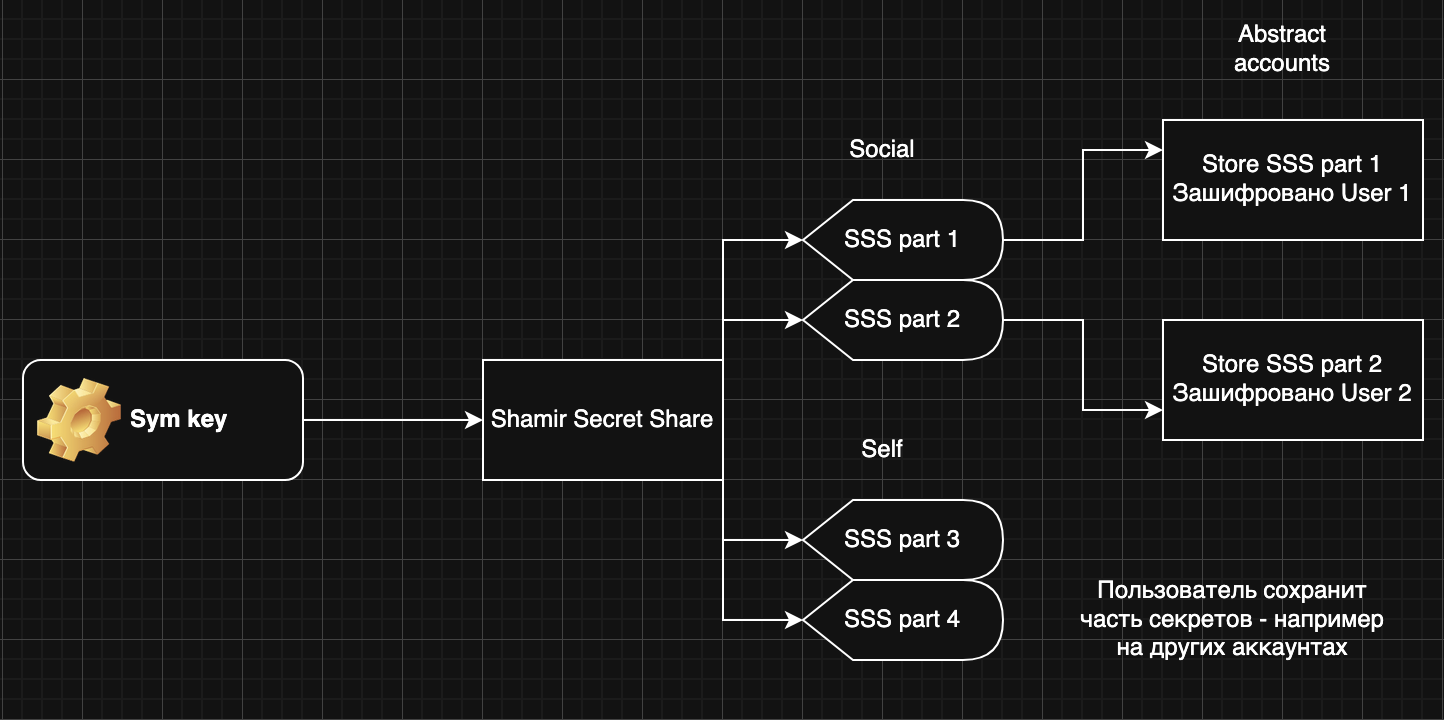
\includegraphics[width=0.8\textwidth]{scheme1}
\caption{Архитектура системы распределения симметричного ключа с использованием алгоритма Шамира}
\label{fig:shamir_scheme}
\end{figure}

На рис.~\ref{fig:shamir_scheme} представлена общая архитектура предлагаемой системы. Симметричный ключ (Sym key) обрабатывается алгоритмом Shamir Secret Sharing, который создает несколько частей секрета (SSS part 1, 2, 3, 4). Эти части распределяются между различными участниками системы: часть передается социальным guardians (которые хранят зашифрованные части в абстрактных аккаунтах), а часть может сохраняться самим пользователем на других устройствах или аккаунтах. Такое распределение обеспечивает отказоустойчивость системы при сохранении конфиденциальности исходного ключа.

Архитектура обеспечивает децентрализованное хранение частей секрета при сохранении возможности восстановления. Предлагаемая схема обеспечивает устойчивость к отказу до $n-k$ guardians и компрометации до $k-1$ guardians одновременно.

\subsection{Компоненты системы}

Система состоит из следующих основных компонентов:
\begin{enumerate}
\item
смарт-контракт на базе CosmWasm, хранящий зашифрованные данные пользователя и метаданные восстановления;
\item
публичный ключ владельца аккаунта для верификации операций;
\item
список доверенных агентов (guardians) с определенным пороговым количеством для восстановления;
\item
механизм сборки секрета через агрегированные подписи guardians при инициации процедуры восстановления.
\end{enumerate}


\section{Детали реализации}

Реализация основана на расширении смарт-контракта абстрактного аккаунта с интеграцией компонентов для работы со схемой Шамира и управления guardians. Исходный код опубликован в открытом репозитории на GitHub.

\subsection{Структура данных смарт-контракта}

Смарт-контракт реализован на языке Rust с использованием фреймворка CosmWasm. Состояние контракта включает следующие ключевые элементы хранения:

\begin{itemize}
\item
\texttt{GUARDIANS}: список адресов доверенных агентов (\texttt{Vec<Addr>});
\item
\texttt{THRESHOLD}: пороговое количество голосов для восстановления (\texttt{u64});
\item
\texttt{VOTES}: карта голосов guardians с их подписями (\texttt{Map<\&Addr, Binary>});
\item
\texttt{COUNTS}: счетчик голосов по каждому новому ключу (\texttt{Map<\&str, u64>});
\item
\texttt{KEY\_VALUE\_STORE}: общее хранилище данных пользователя (\texttt{Map<\&str, Binary>});
\item
\texttt{DATA\_SECRET}: зашифрованный симметричный ключ (\texttt{Binary});
\item
\texttt{SHARES}: части секрета по схеме Шамира для каждого guardian (\texttt{Map<\&Addr, Binary>});
\item
\texttt{RECOVER\_DATA}: временные данные для процесса восстановления (\texttt{Map<\&Addr, Binary>}).
\end{itemize}

Смарт-контракт управляет метаданными и координирует голосование, а криптографические операции выполняются на стороне клиента.

\subsection{Механизм разделения и хранения секрета}

Процесс разделения и распределения секрета включает следующие этапы:

\begin{enumerate}
\item
Исходный симметричный ключ разделяется на $n$ частей с помощью алгоритма Шамира с пороговым значением $k$.

\item
Каждая часть секрета шифруется публичным ключом соответствующего guardian для обеспечения конфиденциальности.

\item
Зашифрованные части сохраняются в абстрактных аккаунтах каждого guardian в поле \texttt{SHARES}.

\item
Каждая сохраненная часть подписывается публичным ключом guardian для обеспечения аутентичности и целостности данных.
\end{enumerate}

\subsection{Алгоритм восстановления секрета}

Процесс восстановления реализован через систему голосования guardians и включает следующие этапы:

\begin{enumerate}
\item
Пользователь инициирует запрос на восстановление, вызывая функцию \texttt{Recover\{new\_pubkey\}} через любого из guardians.

\item
Guardian вызывает функцию \texttt{recover()}, которая проверяет его статус, отсутствие повторного голосования и увеличивает счетчик голосов.

\item
При достижении порогового количества голосов (\texttt{count >= threshold}) происходит автоматическое обновление публичного ключа аккаунта и очистка временных данных голосования.

\item
Guardians могут отозвать свой голос с помощью функции \texttt{Revoke\{\}}, что уменьшает счетчик и удаляет их голос из системы.

\item
Guardians размещают свои части секрета через функции \texttt{StoreShare\{\}} и \texttt{StoreRecoverData\{\}}.

\item
Когда в \texttt{RECOVER\_DATA} накапливается достаточное количество частей, клиентское приложение собирает их и восстанавливает исходный ключ шифрования.
\end{enumerate}

Система предотвращает повторное голосование и обеспечивает атомарность через механизм подсчета голосов.

\subsection{Особенности реализации}

\paragraph{Клиентская часть.}

Пользовательский интерфейс реализован на React с использованием Chakra UI и Cosmos Kit. Основной интерфейс (рис.~\ref{fig:account_interface}) включает управление балансом, guardians и данными.

\begin{figure}[h!] \centering
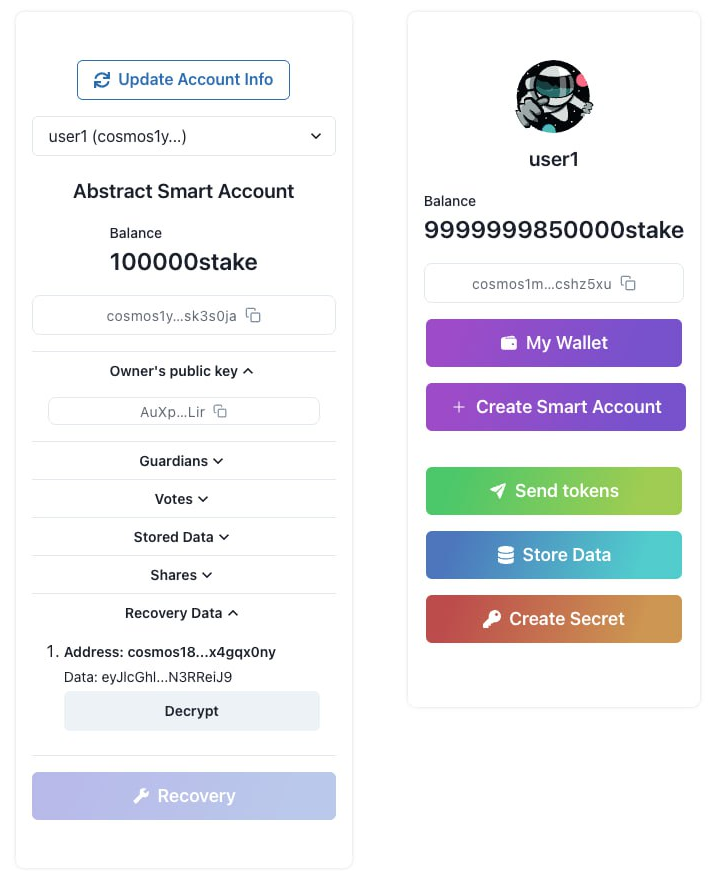
\includegraphics[width=0.7\textwidth]{image3}
\caption{Интерфейс абстрактного аккаунта с функциями управления guardians, голосования и хранения данных}
\label{fig:account_interface}
\end{figure}

\begin{figure}[h!] \centering
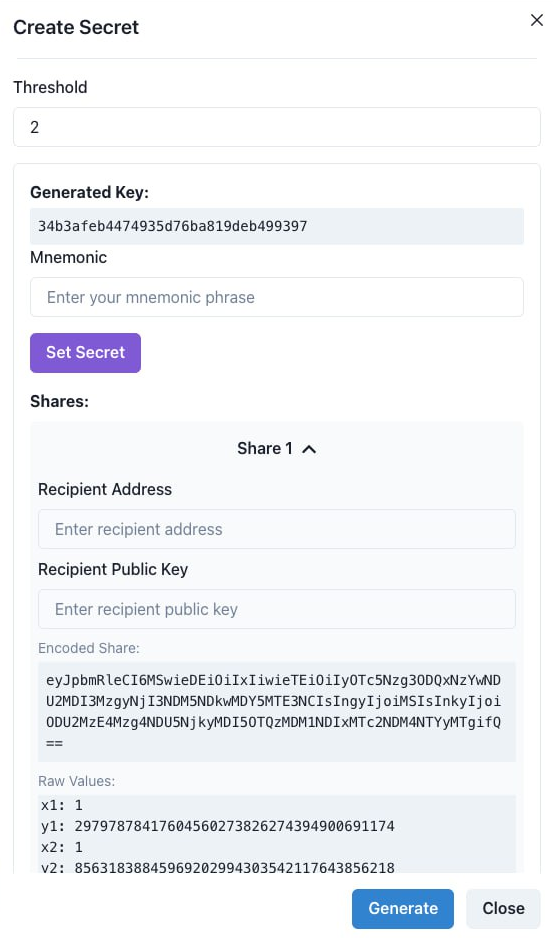
\includegraphics[width=0.7\textwidth]{image4}
\caption{Интерфейс создания и распределения секрета с использованием схемы Шамира}
\label{fig:secret_creation}
\end{figure}

Ключевые компоненты включают \texttt{CreateSecretButton} для генерации и распределения секрета по схеме Шамира, \texttt{WalletSection} для взаимодействия с абстрактным аккаунтом и API-эндпоинт \texttt{/api/generate-shares} для серверной генерации частей секрета. Процесс создания секрета (рис.~\ref{fig:secret_creation}) позволяет пользователю задать пороговое значение, ввести мнемоническую фразу и настроить параметры для каждого guardian.

Процесс создания секрета включает:
\begin{enumerate}
\item
Пользователь указывает количество частей (\texttt{numShares}) и пороговое значение (\texttt{threshold}).
\item
Система генерирует криптографический ключ и разделяет его на части с использованием схемы Шамира.
\item
Каждая часть кодируется в base64 и может быть зашифрована асимметричным ключом соответствующего guardian.
\item
Части сохраняются в смарт-контракте через функцию \texttt{StoreShare}.
\end{enumerate}

\paragraph{Криптографические операции.}

Интеграция схемы Шамира выполняется на стороне клиента для обеспечения конфиденциальности. Используется библиотека \texttt{@cosmjs/crypto} с алгоритмом Secp256k1 для:
\begin{itemize}
\item
генерации ключевых пар из мнемонических фраз;
\item
асимметричного шифрования частей секрета для каждого guardian;
\item
подписи транзакций и верификации подлинности операций.
\end{itemize}

Смарт-контракт хранит только зашифрованные данные и координирует восстановление, не имея доступа к расшифрованной информации.

\section{Анализ безопасности и ограничений}

\subsection{Формальные свойства безопасности}

Безопасность предлагаемой системы обеспечивается математическими свойствами схемы Шамира и архитектурными решениями:

\begin{itemize}
\item
\textbf{Совершенная секретность}: Для схемы $(k,n)$-Шамира любая коалиция из менее чем $k$ участников не получает никакой информации о секрете. Формально, для любых $k-1$ частей $\{s_{i_1}, s_{i_2}, \ldots, s_{i_{k-1}}\}$ и любого возможного секрета $S'$, существует единственный полином степени $k-1$, проходящий через эти точки и имеющий $S'$ в качестве свободного члена.

\item
\textbf{Отказоустойчивость}: Система остается функциональной при недоступности до $n-k$ guardians. При конфигурации $(3,5)$ система выдерживает отказ любых двух участников.

\item
\textbf{Верифицируемость}: Каждая часть секрета подписана публичным ключом соответствующего guardian, что позволяет криптографически верифицировать подлинность данных через проверку подписи.
\end{itemize}

\subsection{Количественная оценка рисков}

Вероятностный анализ компрометации системы:

\begin{itemize}
\item
\textbf{Вероятность компрометации}: При независимой вероятности компрометации каждого guardian равной $p$, вероятность компрометации всей системы составляет $P_{comp} = \sum_{i=k}^{n} \binom{n}{i} p^i (1-p)^{n-i}$. Для схемы $(3,5)$ и $p = 0.1$: $P_{comp} = 0.00856$ (0.856\%).

\item
\textbf{Доступность системы}: Вероятность недоступности при независимой вероятности отказа guardian равной $q$ составляет $P_{unavail} = \sum_{i=n-k+1}^{n} \binom{n}{i} q^i (1-q)^{n-i}$. Для $q = 0.2$: $P_{unavail} = 0.05792$ (5.792\%).
\end{itemize}

\subsection{Архитектурные ограничения}

Выявлены следующие системные ограничения:

\begin{itemize}
\item
\textbf{Социальная инженерия}: Атакующий может попытаться скоординированно воздействовать на $k$ guardians. Противодействие: географическое и социальное разнесение участников, использование институциональных guardians.

\item
\textbf{Доступность данных}: Система требует онлайн-доступности минимум $k$ guardians для восстановления. Решение: избыточность ($n > k$) и мониторинг доступности участников.

\item
\textbf{Временные окна атак}: Период между инициацией восстановления и его завершением создает окно уязвимости. Защита: временные ограничения на операции восстановления и механизмы отмены.
\end{itemize}

\section{Экспериментальная оценка}

Предложенное решение реализовано в виде прототипа на локальной тестовой сети Cosmos SDK. Работоспособность системы подтверждена экспериментально; исходный код смарт-контрактов CosmWasm и клиентского приложения опубликован в открытом доступе.

\subsection{Архитектурные преимущества}

Сравнительный анализ архитектурных особенностей предложенного решения с существующими подходами представлен в табл.~2.

\begin{table}[h]
\begin{flushright}
{Т а б л и ц а 2}\\
\centering
\textbf{Сравнительный анализ архитектурных характеристик}
\end{flushright}
\centering
\begin{tabular}{|l|c|c|c|}
\hline
\textbf{Характеристика} & \textbf{Данная работа} & \textbf{Argent} & \textbf{Pedin~\cite{s15}} \\
\hline
Восстанавливается & Данные + Аккаунт & Аккаунт & Аккаунт \\
\hline
Число транзакций & $k+1$ & $k$ & Константа \\
\hline
Guardians on-chain & Да (голосование) & Да & Нет \\
\hline
Верификация долей & Подписи & Голосование & Merkle Tree \\
\hline
Вычислительная сложность & $O(k^2)$ & $O(k)$ & $O(k^2)$ \\
\hline
Платформа & Cosmos & Ethereum & Ethereum \\
\hline
\end{tabular}
\end{table}

Ключевые особенности предложенной архитектуры:

\begin{itemize}
\item
\textbf{Восстановление данных}: в отличие от Argent (аккаунт) и Pedin (активы), система восстанавливает зашифрованные пользовательские данные, что расширяет область применения за пределы управления средствами.

\item
\textbf{Децентрализация}: полная независимость от централизованных сервисов и Web2-провайдеров; guardians представляют собой независимые аккаунты в блокчейне Cosmos.

\item
\textbf{Вычислительная эффективность}: сложность восстановления секрета через интерполяцию Лагранжа составляет $O(k^2)$, где $k$~--- пороговое значение; для практических конфигураций ($k \leq 10$) издержки приемлемы.

\item
\textbf{Масштабируемость}: архитектура поддерживает динамическое изменение набора guardians без перераспределения всех долей секрета; добавление нового guardian требует только генерации одной новой доли.

\item
\textbf{Гибкость развертывания}: благодаря архитектуре Cosmos SDK, решение может быть развернуто как в публичных сетях (с соответствующими затратами газа), так и в приватных корпоративных блокчейнах с настраиваемыми параметрами производительности.
\end{itemize}

\subsection{Анализ безопасности}

Теоретический анализ безопасности (раздел~5) подтверждает, что система сохраняет конфиденциальность при компрометации до $k-1$ guardians и остаётся функциональной при отказе до $n-k$ участников. Для конфигурации $(3,5)$ вероятность компрометации при независимой вероятности компрометации каждого guardian $p=0.1$ составляет:

$$P_{comp} = \sum_{i=3}^{5} \binom{5}{i} p^i (1-p)^{5-i} \approx 0.00856$$

что обеспечивает высокий уровень защиты ($<$1\% риск компрометации).

\section{Направления дальнейших исследований}

Предложенная архитектура открывает следующие перспективные направления развития:

\begin{enumerate}
\item
\textbf{Прикладные сценарии}: адаптация для корпоративного управления ключами, резервного копирования криптовалютных кошельков и управления доступом к конфиденциальным документам в распределённых системах.

\item
\textbf{Гибридные модели доверия}: интеграция с Web2 OAuth-провайдерами в качестве дополнительного слоя аутентификации guardians с привязкой к системе DID~\cite{s16}.

\item
\textbf{Zero-knowledge доказательства}: верификация корректности вычислений при восстановлении секрета без раскрытия промежуточных данных.

\item
\textbf{Кросс-чейн восстановление}: распределение guardians по различным блокчейн-сетям через IBC и Interchain Accounts для повышения устойчивости.
\end{enumerate}

\section{Заключение}

В данной работе предложена и реализована мультиагентная схема восстановления пользовательских данных в экосистеме Cosmos на основе порогового разделения секрета Шамира.

Ключевые результаты работы:

\begin{enumerate}
\item
В отличие от существующих решений (Argent/Pedin восстанавливают доступ к аккаунту и активам, Leap/Keplr используют централизованный OAuth), предложенная система восстанавливает зашифрованные пользовательские данные через децентрализованную сеть guardians на блокчейне Cosmos без зависимости от Web2.

\item
Доказана устойчивость к компрометации до $k-1$ участников; для конфигурации $(3,5)$ вероятность компрометации $<1\%$ при $p=0.1$. Вычислительная сложность восстановления составляет $O(k^2)$, что приемлемо для $k \leq 10$.

\item
Разработан прототип на CosmWasm с веб-интерфейсом. Открытый исходный код обеспечивает воспроизводимость и развертывание в различных конфигурациях Cosmos-сетей.
\end{enumerate}

Предложенная архитектура расширяет возможности управления данными в Cosmos. Перспективными направлениями являются интеграция с IBC и Interchain Accounts для кросс-чейн сценариев, применение в корпоративных системах, и интеграция с DID для реализации Self-Sovereign Identity.

\themeline

\renewcommand\bibname{Список литературы}
\begin{thebibliography}{99}

\bibitem{s1} \textit{Argent Labs.} Argent: The Most Simple and Safe Crypto Wallet. Argent Documentation. 2023. URL: https://www.argent.xyz

\bibitem{s2} \textit{Buterin V.} EIP-86: Abstraction of transaction origin and signature. Ethereum Improvement Proposals. 2017. URL: https://eips.ethereum.org/EIPS/eip-86

\bibitem{s3} \textit{Buterin V.} EIP-1014: Skinny CREATE2. Ethereum Improvement Proposals. 2018. URL: https://eips.ethereum.org/EIPS/eip-1014

\bibitem{s4} \textit{Buterin V., Dietrichs A., Garnett M., Villanueva W., Wilson S.} EIP-2938: Account Abstraction. Ethereum Improvement Proposals. 2020. URL: https://eips.ethereum.org/EIPS/eip-2938

\bibitem{s5} \textit{Buterin V., Weiss Y., Tirosh D., Nacson S., Forshtat A., Gazso K., Hess T.} ERC-4337: Account Abstraction Using Alt Mempool. Ethereum Improvement Proposals. 2021. URL: https://eips.ethereum.org/EIPS/eip-4337

\bibitem{s6} \textit{CosmWasm Team.} CosmWasm: Smart Contracts for the Cosmos Ecosystem. CosmWasm Documentation. 2021. URL: https://cosmwasm.com

\bibitem{s7} \textit{Ethereum Community.} ERC-7093: Social Recovery Interface. Ethereum Improvement Proposals. 2023. URL: https://eips.ethereum.org/EIPS/eip-7093

\bibitem{s8} \textit{CryptoRank Research Team.} Account Abstraction: Path to Mass Adoption. CryptoRank Insights. 2023. URL: https://cryptorank.io/insights/research/account-abstraction-path-to-mass-adoption

\bibitem{s9} \textit{Buterin V.} Why We Need Wide Adoption of Social Recovery Wallets. Vitalik.ca Blog. 2021. URL: https://vitalik.ca/general/2021/01/11/recovery.html

\bibitem{s10} \textit{Shamir A.} How to share a secret~// Communications of the ACM. 1979. V.~22, N~11. P.~612--613.

\bibitem{s11} \textit{Skibinsky M., Dodis Y., Spies T., Ahmad W.} Decentralized Storage of Crypto Assets via Hierarchical Shamir's Secret Sharing. Vault12 Whitepaper. 2018. URL: https://github.com/vault12/whitepapers

\bibitem{s12} \textit{Miller A.} Simple Security with Shamir Secret Sharing. Grid+ Blog. 2017. URL: https://blog.gridplus.io/simple-security-with-shamir-secret-sharing

\bibitem{s13} \textit{Bartolucci S., Bernat P., Joseph D.} Sharvot: Secret Share-Based Voting on the Blockchain~// WETSEB '18: Proceedings of the 1st International Workshop on Emerging Trends in Software Engineering for Blockchain. 2018. P.~30--34.

\bibitem{s14} \textit{Singh H.P., Stefanidis K., Kirstein F.} A Private Key Recovery Scheme Using Partial Knowledge~// 2021 11th IFIP International Conference on New Technologies, Mobility and Security (NTMS). Paris, France. 2021. P.~1--5.

\bibitem{s15} \textit{Pedin A.B., Siasi N., Sameni M.} Smart Contract-Based Social Recovery Wallet Management Scheme for Digital Assets~// Proceedings of the 2023 ACM Southeast Conference (ACMSE '23). 2023. P.~177--181.

\bibitem{s16} \textit{Allen C.} The Path to Self-Sovereign Identity. Life With Alacrity Blog. 2016. URL: http://www.lifewithalacrity.com/2016/04/the-path-to-self-soverereign-identity.html

\end{thebibliography}

%References
\selectlanguage{english}
\begin{thebibliography}{99}
\selectlanguage{russian}

\bibitem{s1} \textit{Argent Labs.} Argent: The Most Simple and Safe Crypto Wallet. Argent Documentation. 2023. URL: https://www.argent.xyz

\bibitem{s2} \textit{Buterin V.} EIP-86: Abstraction of transaction origin and signature. Ethereum Improvement Proposals. 2017. URL: https://eips.ethereum.org/EIPS/eip-86

\bibitem{s3} \textit{Buterin V.} EIP-1014: Skinny CREATE2. Ethereum Improvement Proposals. 2018. URL: https://eips.ethereum.org/EIPS/eip-1014

\bibitem{s4} \textit{Buterin V., Dietrichs A., Garnett M., Villanueva W., Wilson S.} EIP-2938: Account Abstraction. Ethereum Improvement Proposals. 2020. URL: https://eips.ethereum.org/EIPS/eip-2938

\bibitem{s5} \textit{Buterin V., Weiss Y., Tirosh D., Nacson S., Forshtat A., Gazso K., Hess T.} ERC-4337: Account Abstraction Using Alt Mempool. Ethereum Improvement Proposals. 2021. URL: https://eips.ethereum.org/EIPS/eip-4337

\bibitem{s6} \textit{CosmWasm Team.} CosmWasm: Smart Contracts for the Cosmos Ecosystem. CosmWasm Documentation. 2021. URL: https://cosmwasm.com

\bibitem{s7} \textit{Ethereum Community.} ERC-7093: Social Recovery Interface. Ethereum Improvement Proposals. 2023. URL: https://eips.ethereum.org/EIPS/eip-7093

\bibitem{s8} \textit{CryptoRank Research Team.} Account Abstraction: Path to Mass Adoption. CryptoRank Insights. 2023. URL: https://cryptorank.io/insights/research/account-abstraction-path-to-mass-adoption

\bibitem{s9} \textit{Buterin V.} Why We Need Wide Adoption of Social Recovery Wallets. Vitalik.ca Blog. 2021. URL: https://vitalik.ca/general/2021/01/11/recovery.html

\bibitem{s10} \textit{Shamir A.} How to share a secret. Communications of the ACM. 1979. V.~22, N~11. P.~612--613.

\bibitem{s11} \textit{Skibinsky M., Dodis Y., Spies T., Ahmad W.} Decentralized Storage of Crypto Assets via Hierarchical Shamir's Secret Sharing. Vault12 Whitepaper. 2018. URL: https://github.com/vault12/whitepapers

\bibitem{s12} \textit{Miller A.} Simple Security with Shamir Secret Sharing. Grid+ Blog. 2017. URL: https://blog.gridplus.io/simple-security-with-shamir-secret-sharing

\bibitem{s13} \textit{Bartolucci S., Bernat P., Joseph D.} Sharvot: Secret Share-Based Voting on the Blockchain. WETSEB '18: Proceedings of the 1st International Workshop on Emerging Trends in Software Engineering for Blockchain. 2018. P.~30--34.

\bibitem{s14} \textit{Singh H.P., Stefanidis K., Kirstein F.} A Private Key Recovery Scheme Using Partial Knowledge. 2021 11th IFIP International Conference on New Technologies, Mobility and Security (NTMS). Paris, France. 2021. P.~1--5.

\bibitem{s15} \textit{Pedin A.B., Siasi N., Sameni M.} Smart Contract-Based Social Recovery Wallet Management Scheme for Digital Assets. Proceedings of the 2023 ACM Southeast Conference (ACMSE '23). 2023. P.~177--181.

\bibitem{s16} \textit{Allen C.} The Path to Self-Sovereign Identity. Life With Alacrity Blog. 2016. URL: http://www.lifewithalacrity.com/2016/04/the-path-to-self-soverereign-identity.html

\end{thebibliography}
\selectlanguage{russian}

\begin{flushright}
Поступила в редакцию дд.мм.гггг
\end{flushright}
